\documentclass[12pt,a4paper]{article}

% Packages
\usepackage[utf8]{inputenc}
\usepackage[T1]{fontenc}
\usepackage{graphicx}
\usepackage{geometry}
\usepackage{hyperref}
\usepackage{xcolor}
\usepackage{booktabs}
\usepackage{enumitem}
\usepackage{fancyhdr}
\usepackage{titlesec}
\usepackage{float}

% Page geometry
\geometry{margin=1in}

% Colors
\definecolor{criticalred}{RGB}{220, 53, 69}
\definecolor{warningorange}{RGB}{255, 193, 7}
\definecolor{enhancementblue}{RGB}{23, 162, 184}
\definecolor{sectioncoral}{RGB}{205, 92, 92}

% Hyperlink setup
\hypersetup{
    colorlinks=true,
    linkcolor=sectioncoral,
    urlcolor=blue,
    citecolor=black
}

% Header/Footer
\pagestyle{fancy}
\fancyhf{}
\rhead{Together SwarmSpace Review}
\lhead{Website UX Analysis}
\rfoot{Page \thepage}

% Title formatting
\titleformat{\section}
  {\normalfont\Large\bfseries\color{sectioncoral}}{\thesection}{1em}{}
\titleformat{\subsection}
  {\normalfont\large\bfseries}{\thesubsection}{1em}{}

\begin{document}

% Title Page
\begin{titlepage}
    \centering
    \vspace*{2cm}
    
    {\Huge\bfseries Comprehensive UX Review\\[0.5cm]}
    {\LARGE Together SwarmSpace Website\\[1cm]}
    
    \vspace{1cm}
    
    {\large\texttt{https://www.together.fund/togetherswarmspace}}
    
    \vspace{2cm}
    
    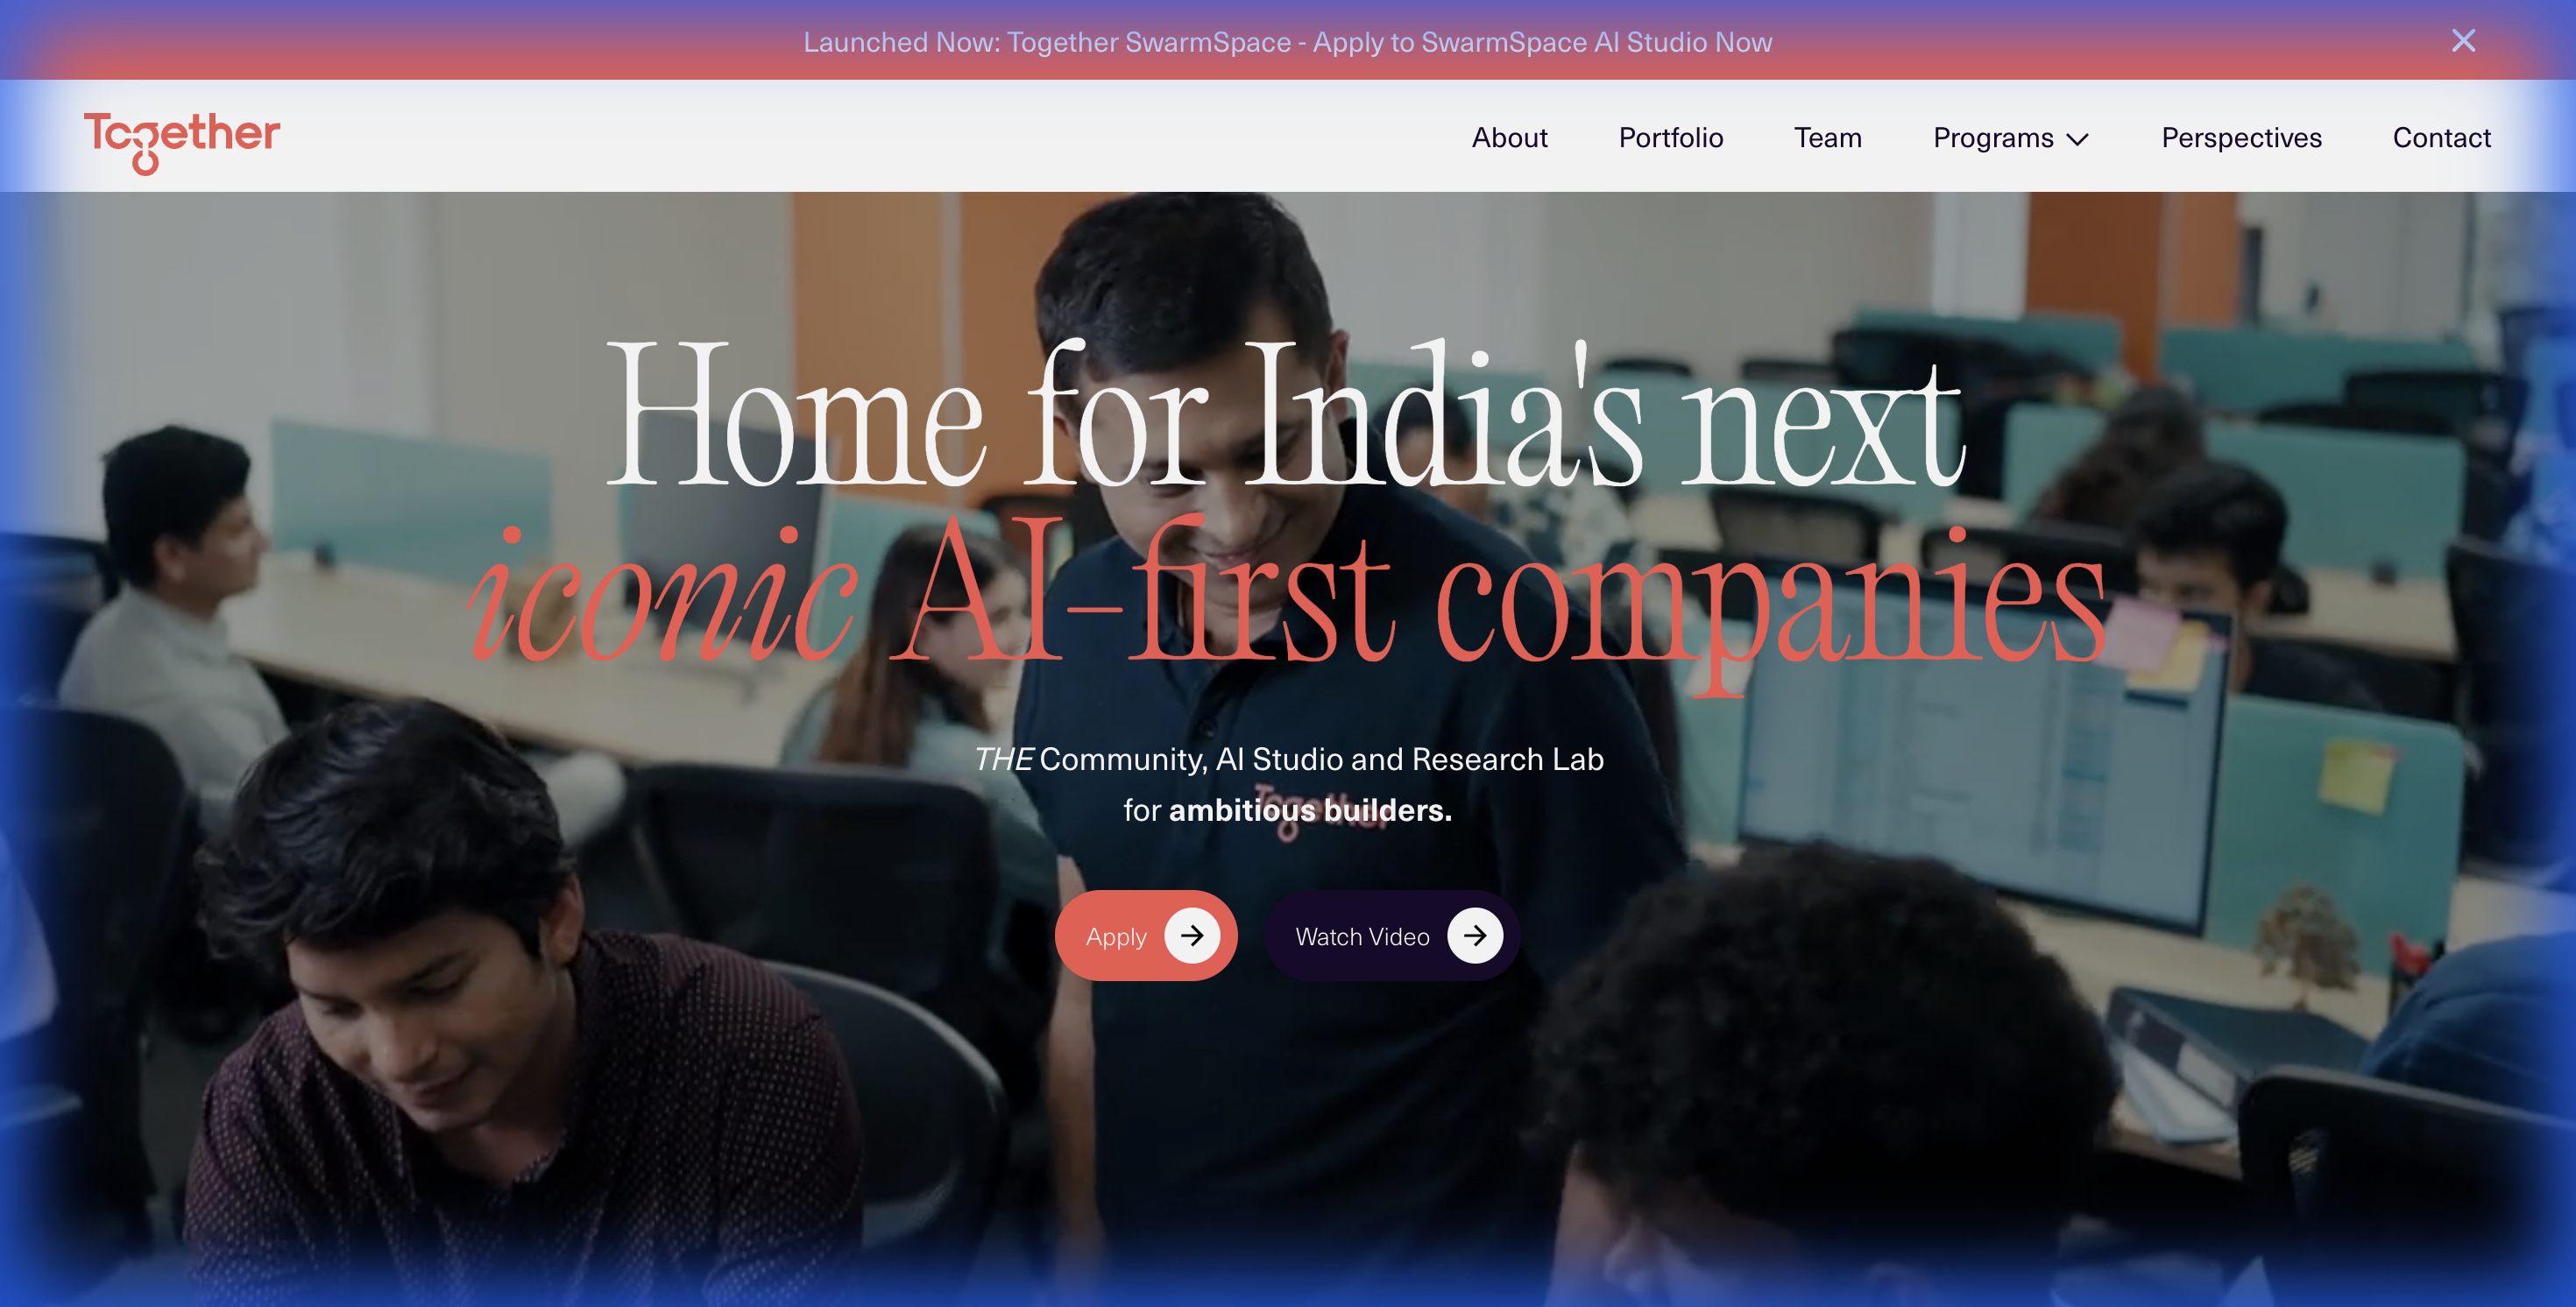
\includegraphics[width=0.9\textwidth]{hero_section.png}
    
    \vfill
    
    {\large\textbf{Document Date:} January 17, 2026}\\[0.5cm]
    {\large\textbf{Review Type:} Landing Page UX/UI Analysis}
    
\end{titlepage}

% Table of Contents
\tableofcontents
\newpage

% ============================================
\section{Executive Summary}
% ============================================

The Together SwarmSpace website presents a \textbf{polished, professional aesthetic} with a warm cream background, coral-red accent color, and sophisticated typography combining serif headings with sans-serif body text. 

However, several \textbf{structural and UX issues} limit its effectiveness as a landing page for an AI accelerator program. This document provides a comprehensive analysis of issues and recommended improvements, organized by priority level.

\subsection{Key Findings at a Glance}

\begin{itemize}[leftmargin=*]
    \item \textbf{4 Critical Issues} requiring immediate attention
    \item \textbf{5 Medium Priority} improvements for better UX
    \item \textbf{4 Enhancement Suggestions} for a polished experience
\end{itemize}

\newpage

% ============================================
\section{Visual Overview}
% ============================================

\subsection{Hero Section}

The hero section features a high-impact background video with a clear value proposition: ``Home for India's next iconic AI-first companies.'' The ``Apply'' and ``Watch Video'' CTAs are prominently placed.

\begin{figure}[H]
    \centering
    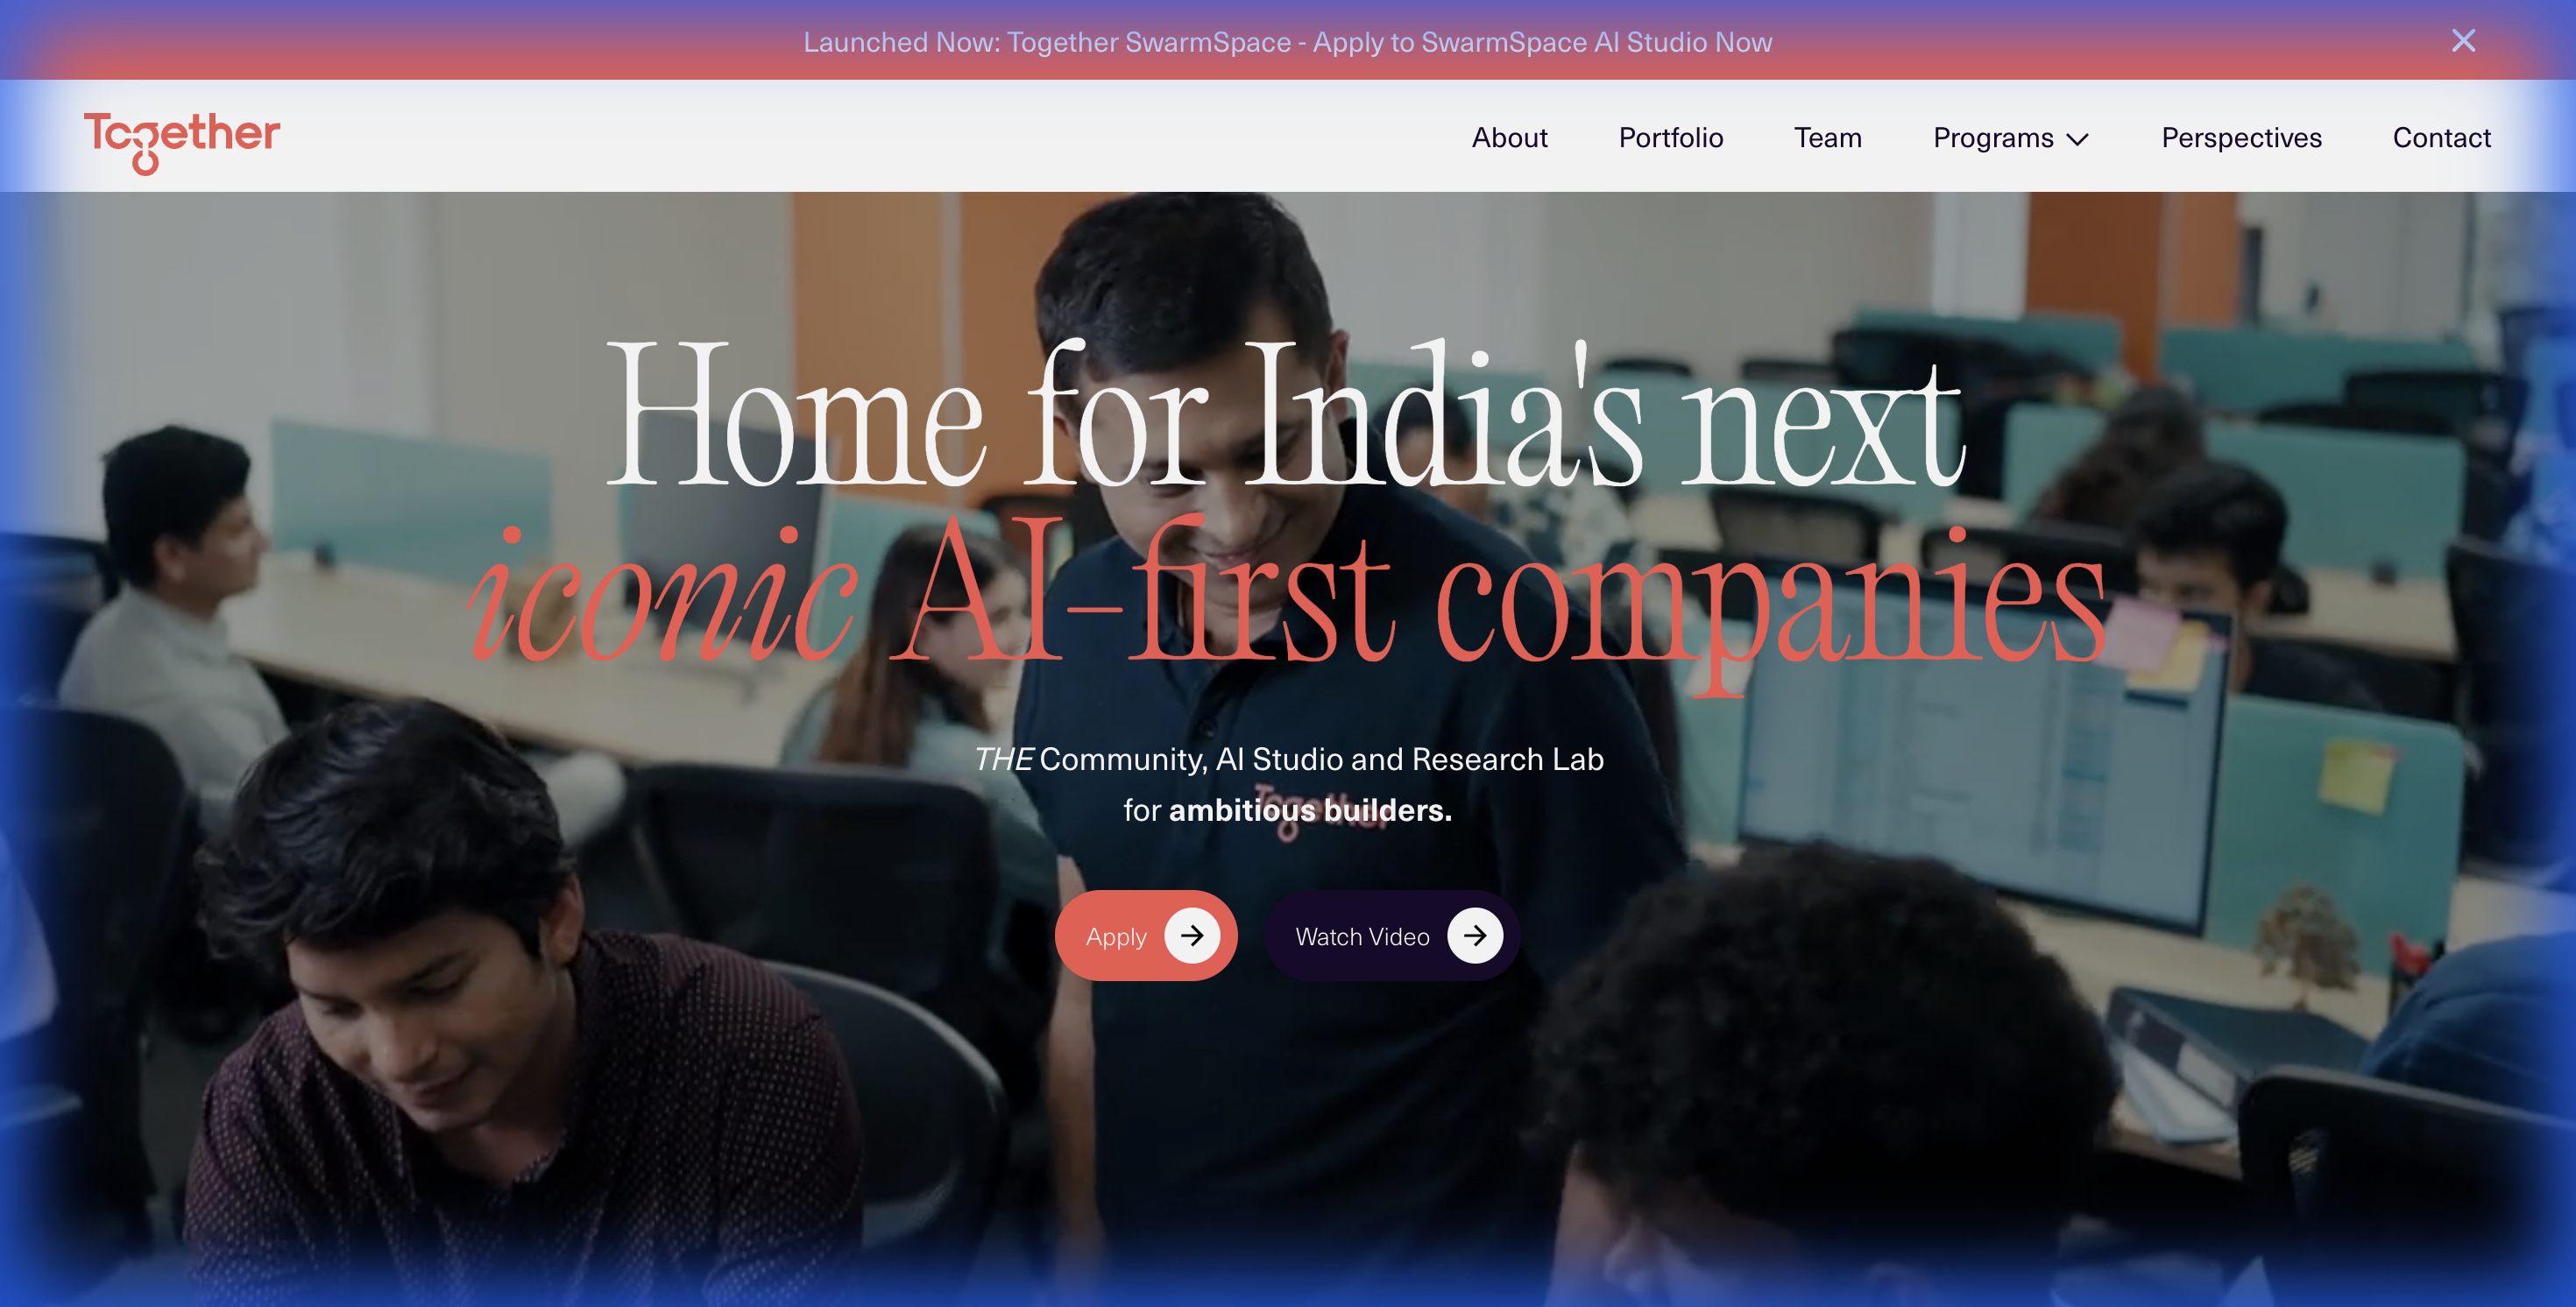
\includegraphics[width=\textwidth]{hero_section.png}
    \caption{Hero section with background video and primary CTAs}
    \label{fig:hero}
\end{figure}

\subsection{Three Pillars Section}

This section introduces the three core offerings: Community, AI Studio, and Research Lab. The sector pills (Foundation Models, AI Infra/Tools, etc.) appear here but are non-interactive.

\begin{figure}[H]
    \centering
    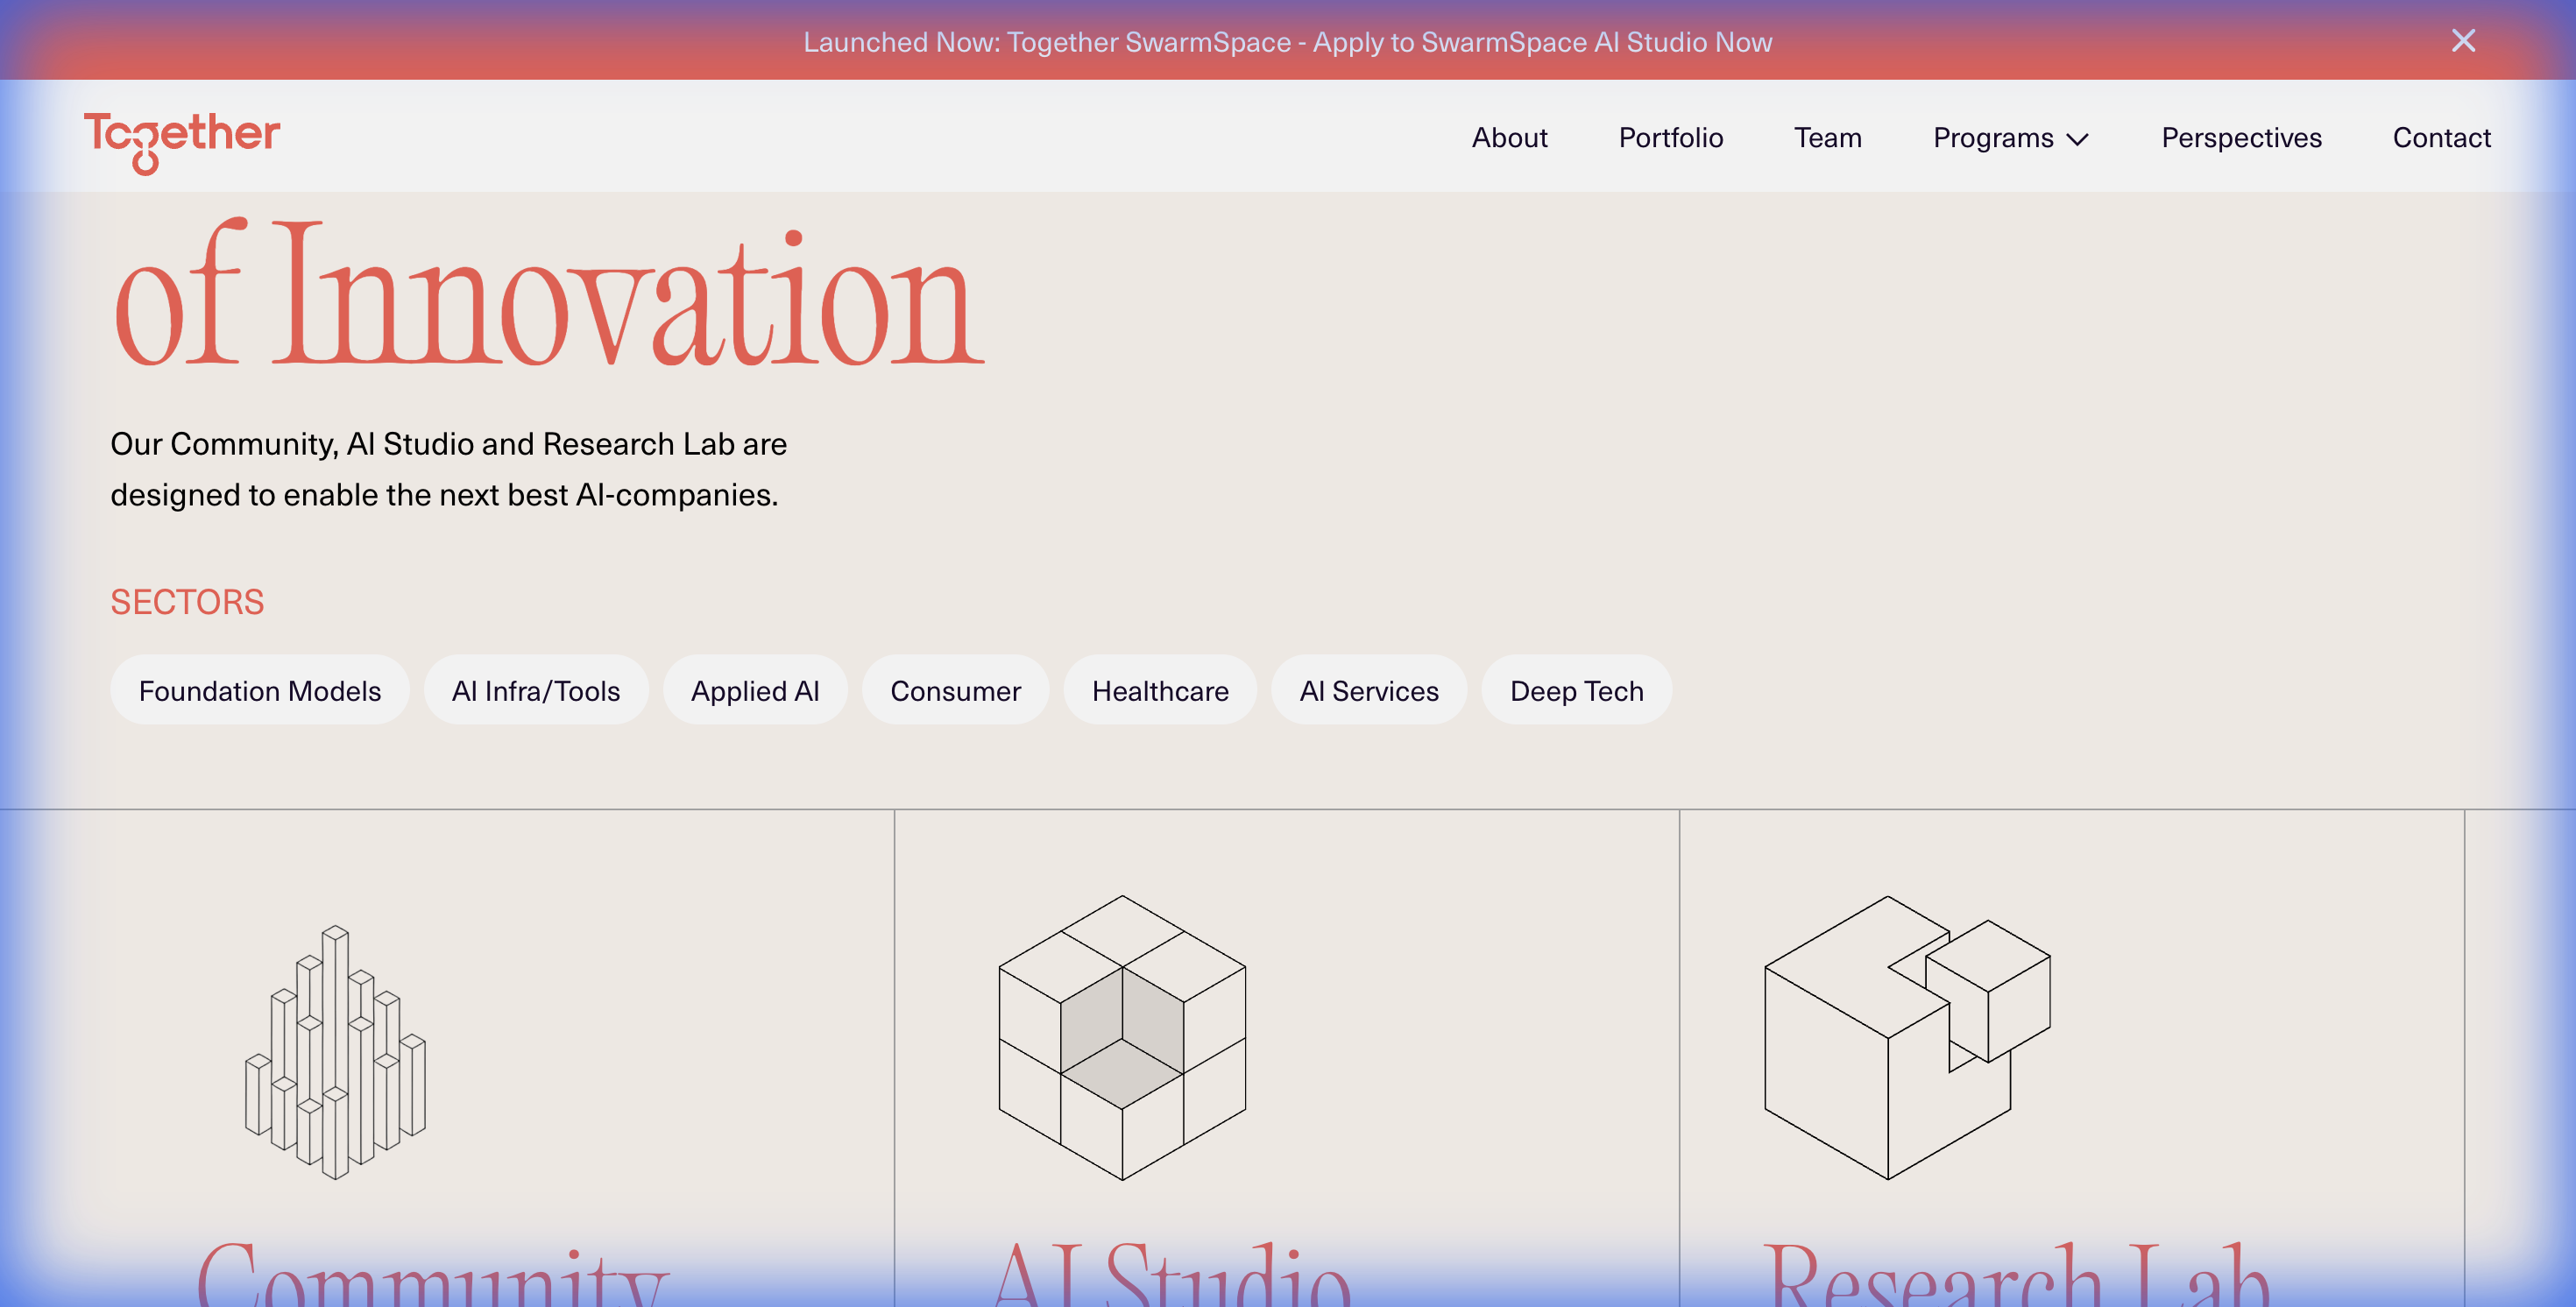
\includegraphics[width=\textwidth]{three_pillars_section.png}
    \caption{Three Pillars of Innovation with sector tags}
    \label{fig:pillars}
\end{figure}

\subsection{Program Details Section}

The ``Program Designed for AI Builders'' section highlights the 12-week intensive program and key benefits.

\begin{figure}[H]
    \centering
    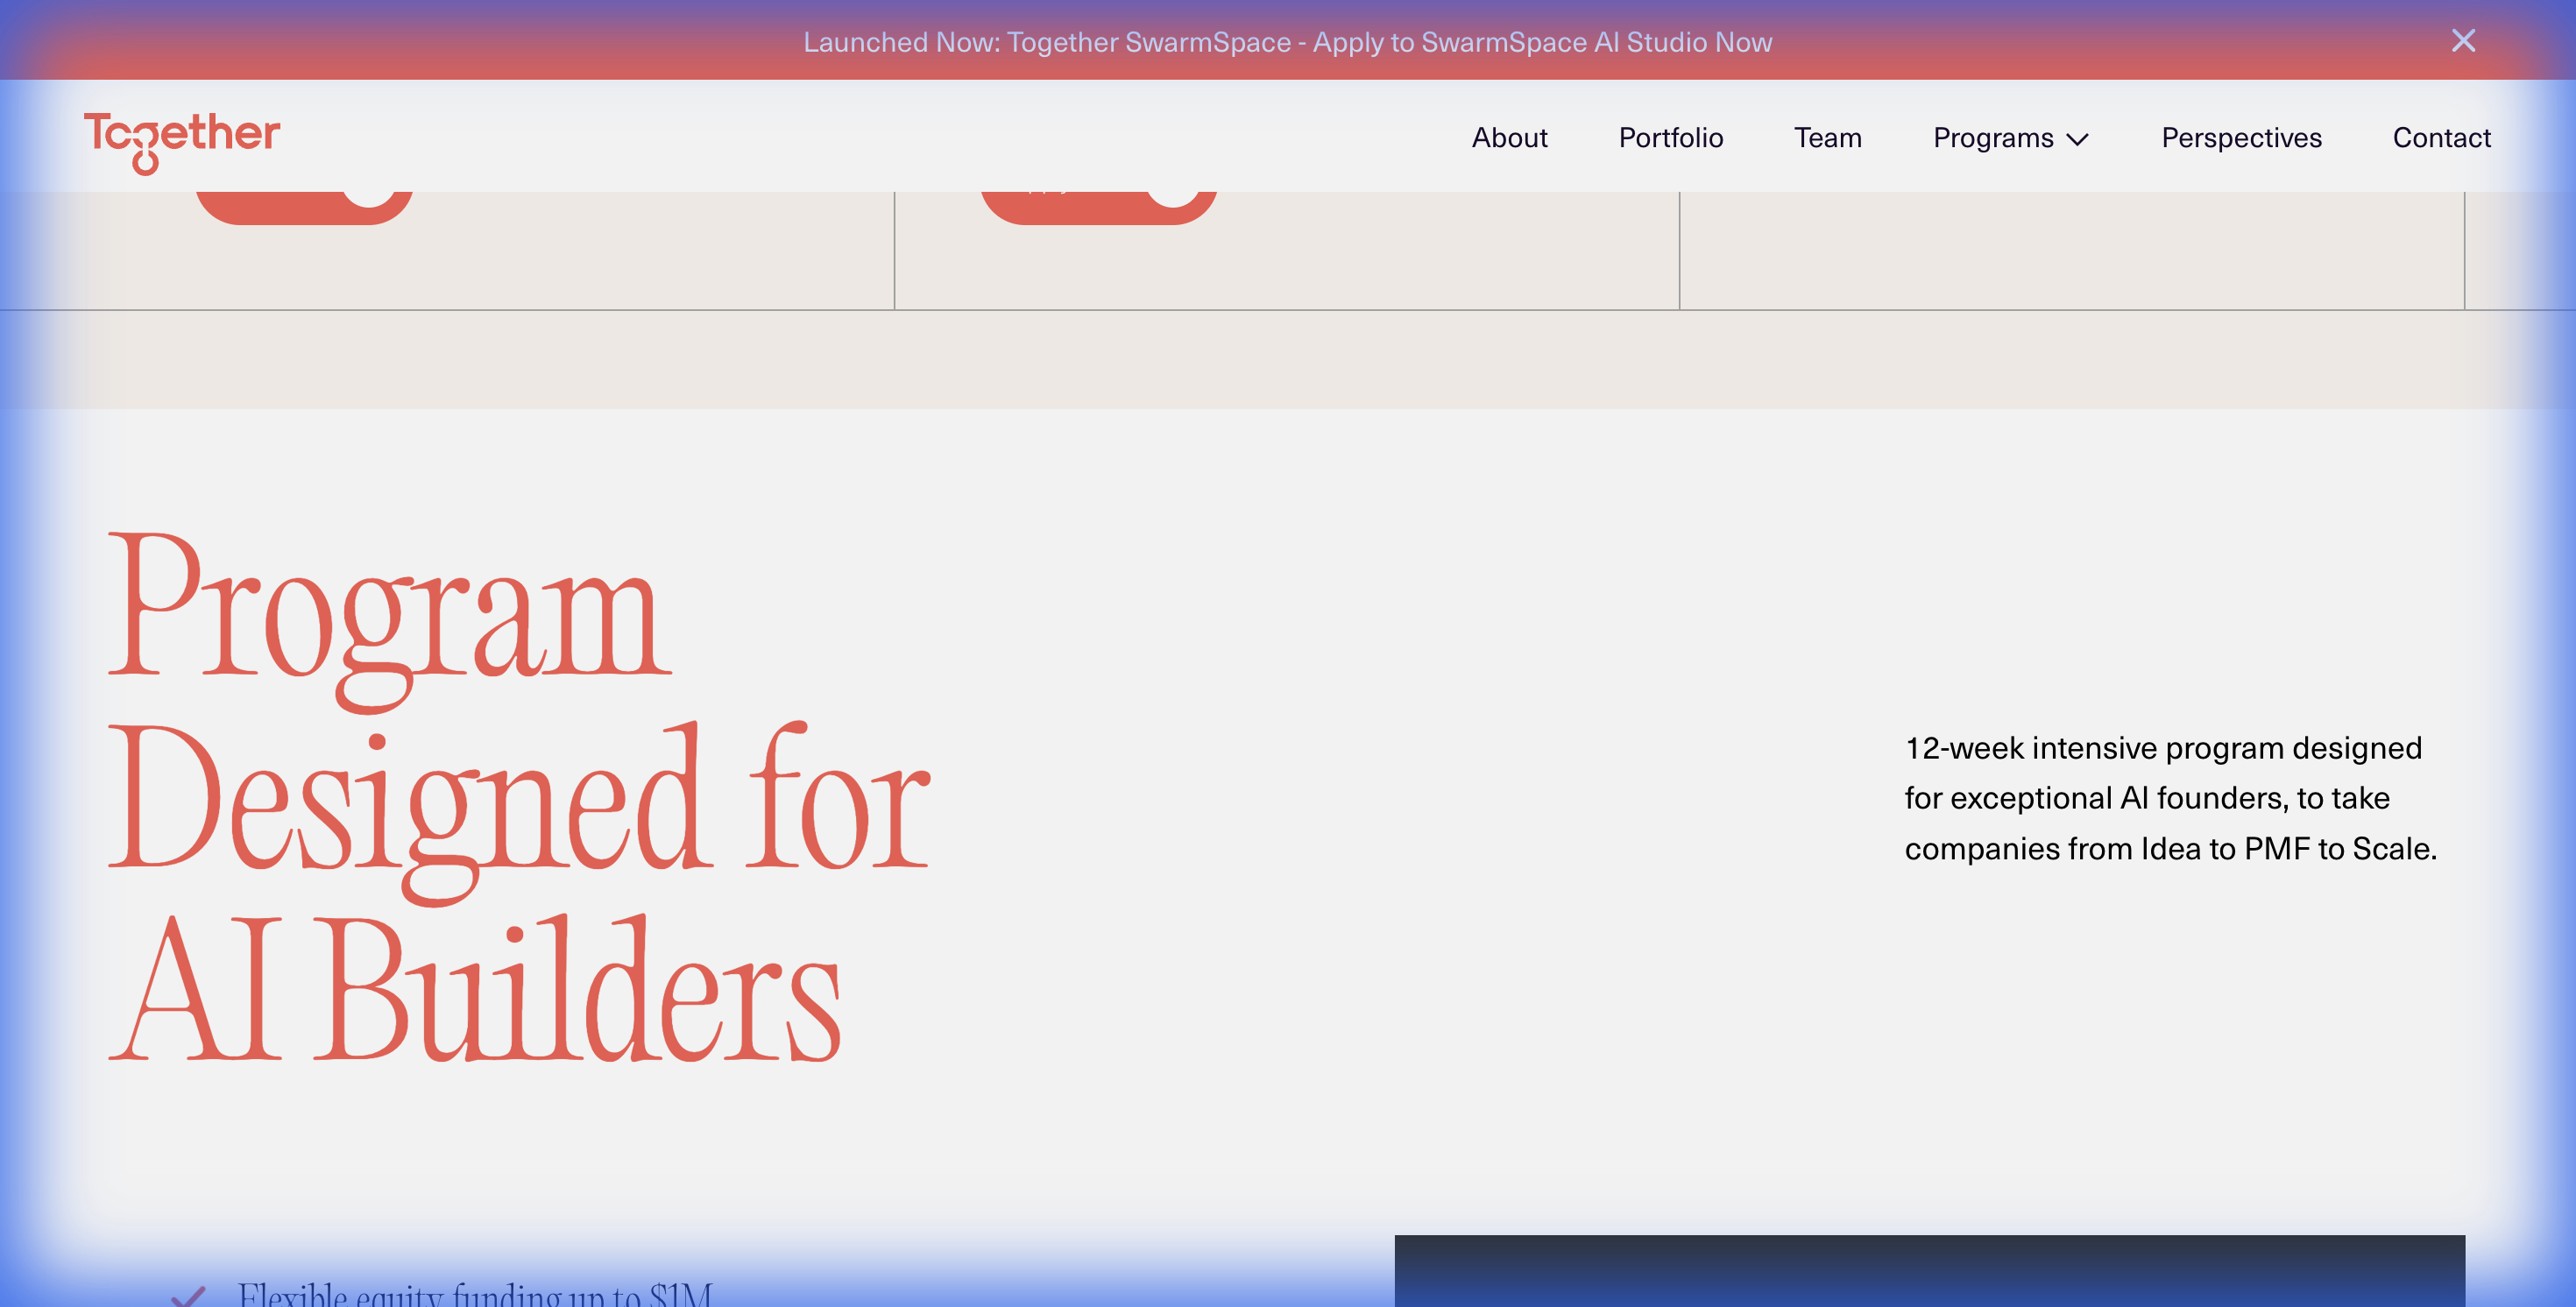
\includegraphics[width=\textwidth]{program_designed_section.png}
    \caption{Program benefits and partner logos}
    \label{fig:program}
\end{figure}

\subsection{FAQ Section}

Standard accordion-style FAQ section addressing common questions about the program.

\begin{figure}[H]
    \centering
    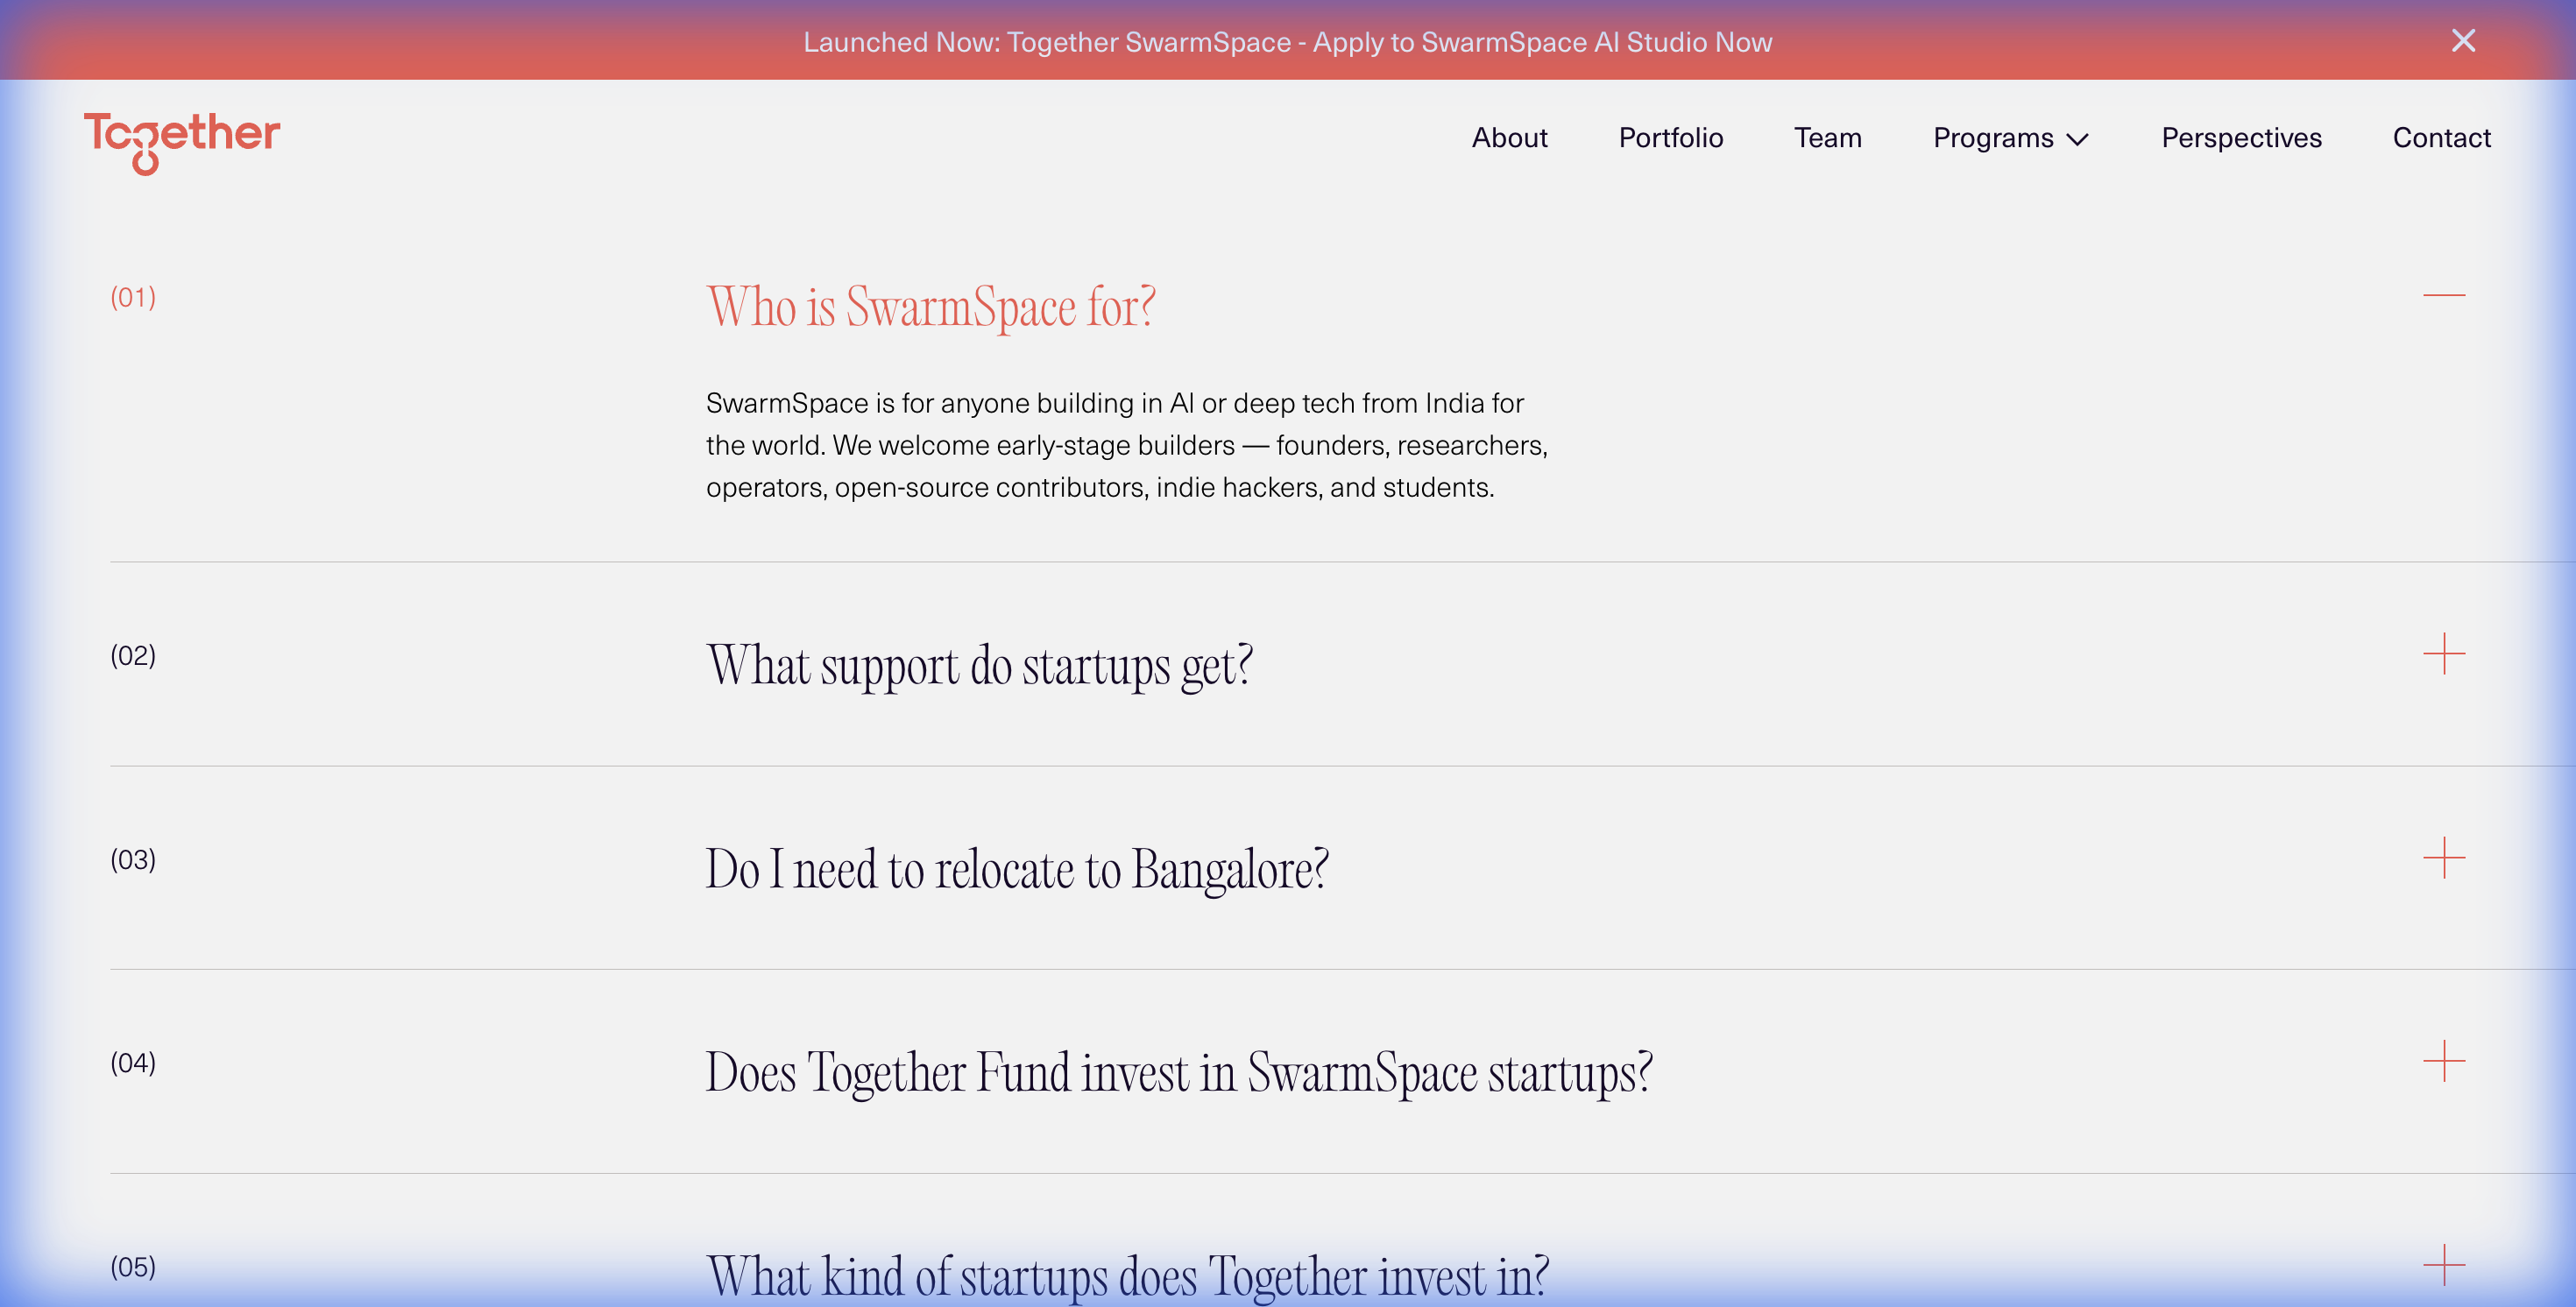
\includegraphics[width=\textwidth]{faq_footer_section.png}
    \caption{Frequently Asked Questions section}
    \label{fig:faq}
\end{figure}

\newpage

% ============================================
\section{Critical Issues}
\textcolor{criticalred}{\rule{\linewidth}{2pt}}
% ============================================

These issues significantly impact user experience and conversion potential. They should be addressed immediately.

\subsection{Issue 1: Lack of Context --- ``What is SwarmSpace?''}

\begin{description}[leftmargin=!,labelwidth=\widthof{\bfseries Problem:}]
    \item[Problem:] The landing page assumes visitors already know what SwarmSpace is. There is no dedicated introduction section explaining the accelerator program's unique value proposition.
    
    \item[Impact:] First-time visitors (the primary target audience) may be confused about what they're signing up for.
    
    \item[Evidence:] User feedback: ``What is SwarmSpace randomly'' / ``Not enough context''
    
    \item[Recommendation:] Add a prominent ``What is SwarmSpace?'' section immediately after the hero, with a 2-3 sentence explanation of the accelerator's mission and differentiators.
\end{description}

\subsection{Issue 2: Sectors Are Non-Interactive (Dead UI)}

\begin{description}[leftmargin=!,labelwidth=\widthof{\bfseries Problem:}]
    \item[Problem:] The sector tags (Foundation Models, AI Infra/Tools, Applied AI, Consumer, Healthcare, AI Services, Deep Tech) are static pills with no interactivity.
    
    \item[Impact:] Users naturally expect clickable elements to lead somewhere. This creates a frustrating ``dead end'' experience.
    
    \item[Evidence:] User feedback: ``Sectors should connect to like a detailed blog or list''
    
    \item[Recommendation:] Make each sector clickable, leading to either:
    \begin{itemize}
        \item A filtered portfolio view showing companies in that sector
        \item A dedicated blog post or thesis page explaining Together's investment thesis for that sector
    \end{itemize}
\end{description}

\begin{figure}[H]
    \centering
    \fbox{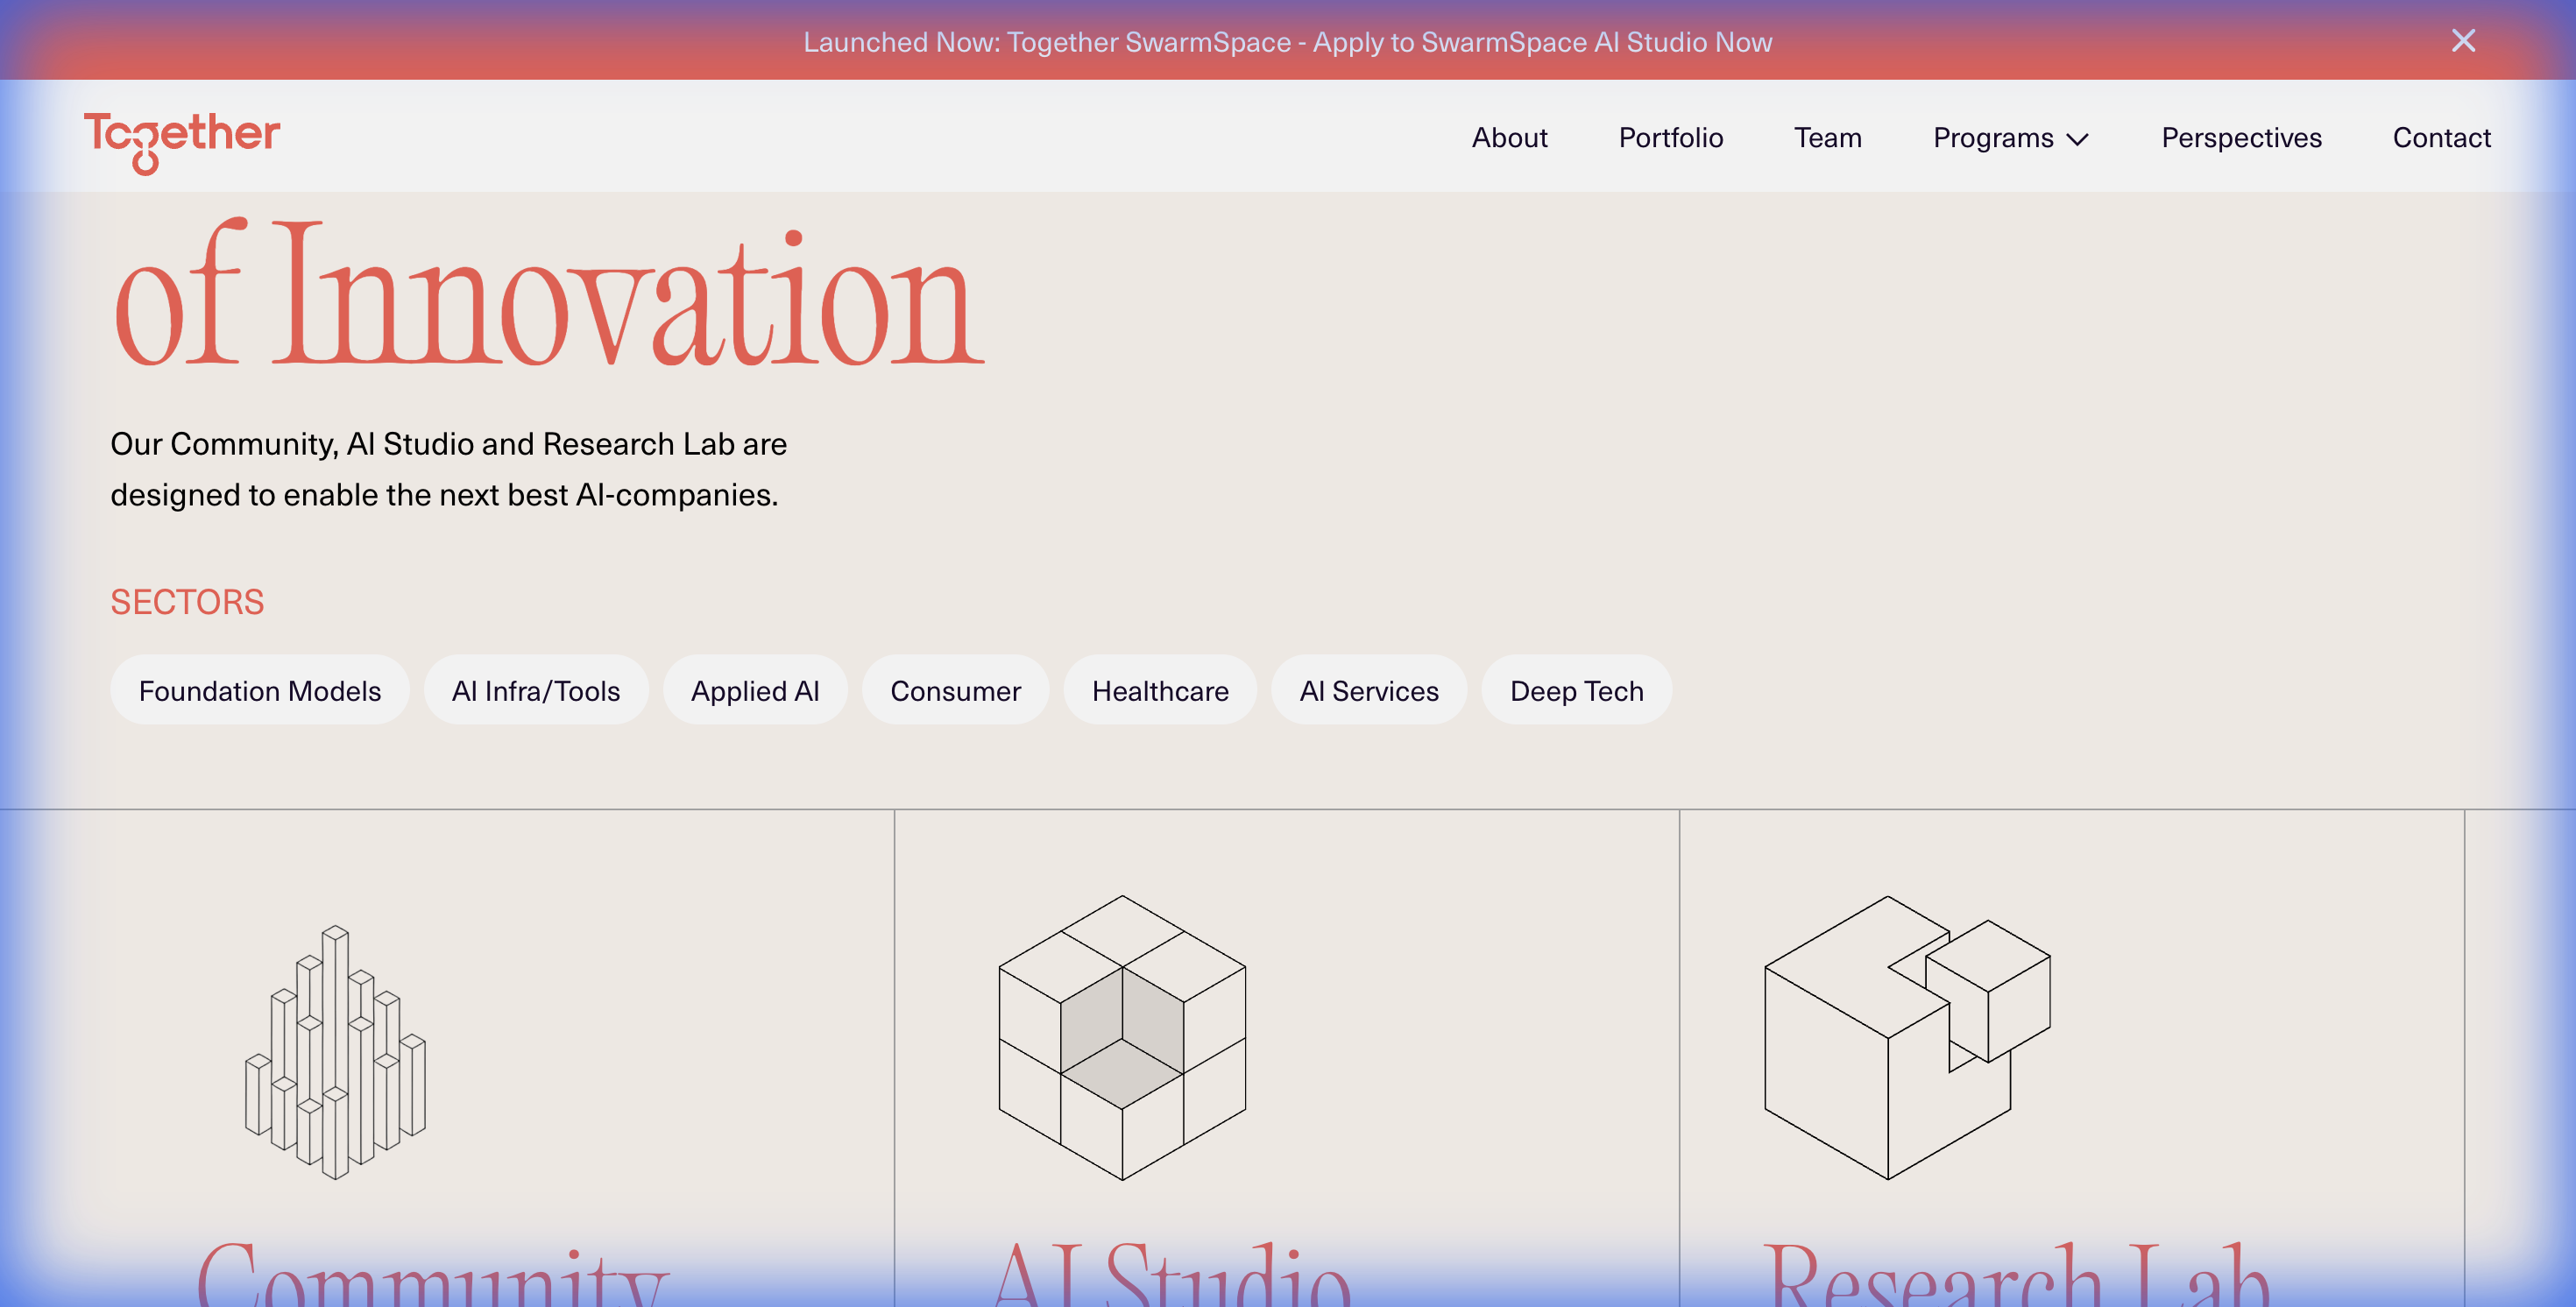
\includegraphics[width=0.8\textwidth]{three_pillars_section.png}}
    \caption{Sector pills highlighted --- currently non-interactive}
    \label{fig:sectors}
\end{figure}

\subsection{Issue 3: Research Lab Has No CTA}

\begin{description}[leftmargin=!,labelwidth=\widthof{\bfseries Problem:}]
    \item[Problem:] The Three Pillars section shows inconsistent CTAs:
    \begin{itemize}
        \item Community $\rightarrow$ ``Join Now'' button
        \item AI Studio $\rightarrow$ ``Apply Now'' button
        \item Research Lab $\rightarrow$ \textbf{No button at all}
    \end{itemize}
    
    \item[Impact:] Inconsistency in UI patterns reduces trust and missed conversion opportunity.
    
    \item[Recommendation:] Add a CTA button such as ``Learn More'' or ``Explore Research'' linking to details about the research program or a contact form.
\end{description}

\subsection{Issue 4: Broken Footer Links}

\begin{description}[leftmargin=!,labelwidth=\widthof{\bfseries Problem:}]
    \item[Problem:] Multiple footer links point incorrectly to the SwarmSpace page itself:
    \begin{itemize}
        \item Privacy Policy $\rightarrow$ SwarmSpace page
        \item Terms of Service $\rightarrow$ SwarmSpace page
        \item Disclaimer $\rightarrow$ SwarmSpace page
        \item Resources $\rightarrow$ SwarmSpace page
        \item Blog $\rightarrow$ SwarmSpace page
        \item Changelog $\rightarrow$ SwarmSpace page
    \end{itemize}
    
    \item[Impact:] This is unprofessional and potentially a legal compliance issue (missing privacy policy).
    
    \item[Recommendation:] Create actual pages for Privacy Policy, ToS, and Disclaimer. Either build out Resources/Blog/Changelog pages or remove these links until ready.
\end{description}

\newpage

% ============================================
\section{Medium Priority Improvements}
\textcolor{warningorange}{\rule{\linewidth}{2pt}}
% ============================================

These issues affect user experience but are not blocking. They should be addressed in the next iteration.

\subsection{Issue 5: ``Program Built for Builders'' Card Visibility}

\begin{description}[leftmargin=!,labelwidth=\widthof{\bfseries Problem:}]
    \item[Problem:] This section contains crucial selling points (up to \$1M funding, 12-week duration, \$600K credits, office space in Bangalore and Palo Alto) but is buried below the fold.
    
    \item[Evidence:] User feedback: ``The program built for builders card can be higher''
    
    \item[Recommendation:] Either:
    \begin{itemize}
        \item Move this section higher in the page hierarchy, OR
        \item Make the Three Pillars section more compact to reduce scroll distance
    \end{itemize}
\end{description}

\subsection{Issue 6: Partner Logos Lack Context}

\begin{description}[leftmargin=!,labelwidth=\widthof{\bfseries Problem:}]
    \item[Problem:] Microsoft, OpenAI, and Google Cloud logos appear at the bottom of the program section without explanation of what they represent.
    
    \item[Impact:] Visitors may assume these are portfolio companies, investors, or random endorsements.
    
    \item[Recommendation:] Add a clear label above the logos such as ``Credits \& Infrastructure Partners'' or ``Powered By.''
\end{description}

\subsection{Issue 7: Global Network Section Is Sparse}

\begin{description}[leftmargin=!,labelwidth=\widthof{\bfseries Problem:}]
    \item[Problem:] Bangalore, Palo Alto, and Chennai locations are mentioned with minimal detail. There are no images, no addresses, and no information about capacity or amenities.
    
    \item[Recommendation:] Enhance with:
    \begin{itemize}
        \item Photos of each office location
        \item A small map or geographical visual
        \item More tangible details (sq ft, amenities, proximity to transit)
    \end{itemize}
\end{description}

\subsection{Issue 8: Portfolio Lacks Sector Categorization}

\begin{description}[leftmargin=!,labelwidth=\widthof{\bfseries Problem:}]
    \item[Problem:] Portfolio companies are listed with one-liner descriptions but no categorization by sector. This doesn't leverage the sector pills shown earlier.
    
    \item[Recommendation:] Allow filtering by sector, or visually group companies by their domain (Healthcare AI, Enterprise AI, etc.).
\end{description}

\subsection{Issue 9: No Social Proof or Success Stories}

\begin{description}[leftmargin=!,labelwidth=\widthof{\bfseries Problem:}]
    \item[Problem:] There are no testimonials from previous cohort founders and no metrics demonstrating program success.
    
    \item[Recommendation:] Add:
    \begin{itemize}
        \item Testimonials carousel from alumni founders
        \item ``By the Numbers'' section (e.g., ``X companies funded, \$Y raised by portfolio'')
    \end{itemize}
\end{description}

\newpage

% ============================================
\section{Enhancement Suggestions}
\textcolor{enhancementblue}{\rule{\linewidth}{2pt}}
% ============================================

These are optional improvements that would elevate the website from good to excellent.

\subsection{Enhancement 1: Timeline / What to Expect Section}

The 12-week program is mentioned but not explained in detail. Founders want to know:
\begin{itemize}
    \item What happens in each phase?
    \item When does the US immersion occur?
    \item What is the weekly time commitment?
\end{itemize}

\textbf{Recommendation:} Add a visual timeline showing the program journey from application to demo day.

\subsection{Enhancement 2: Application Timeline and Deadlines}

Currently, there is no information about:
\begin{itemize}
    \item Application deadlines
    \item Cohort schedules
    \item Selection criteria
    \item What to prepare for the application
\end{itemize}

\textbf{Recommendation:} Add an ``Application Timeline'' section with next cohort dates and deadlines.

\subsection{Enhancement 3: Blog/Perspectives Integration}

The site has a ``Perspectives'' section in the navigation but doesn't leverage this content on the SwarmSpace landing page.

\textbf{Recommendation:} Add a ``Latest Insights'' section showcasing 2-3 relevant blog posts about AI trends, founder advice, or investment theses.

\subsection{Enhancement 4: Embedded Video Preview}

The hero has a ``Watch Video'' button linking to YouTube, requiring users to leave the page.

\textbf{Recommendation:} Consider an inline video player or at least a thumbnail preview with a play button to increase engagement.

\newpage

% ============================================
\section{Summary Checklist}
% ============================================

\begin{table}[H]
\centering
\begin{tabular}{@{}llc@{}}
\toprule
\textbf{Issue} & \textbf{Priority} & \textbf{Status} \\
\midrule
Add ``What is SwarmSpace?'' intro section & \textcolor{criticalred}{Critical} & $\times$ \\
Make sector pills clickable/linked & \textcolor{criticalred}{Critical} & $\times$ \\
Add CTA button to Research Lab & \textcolor{criticalred}{Critical} & $\times$ \\
Fix broken footer links & \textcolor{criticalred}{Critical} & $\times$ \\
\midrule
Elevate ``Program Built for Builders'' section & \textcolor{warningorange}{Medium} & $\circ$ \\
Add context to partner logos & \textcolor{warningorange}{Medium} & $\circ$ \\
Enrich Global Network section with photos & \textcolor{warningorange}{Medium} & $\circ$ \\
Add portfolio filtering by sector & \textcolor{warningorange}{Medium} & $\circ$ \\
Add testimonials/success stories & \textcolor{warningorange}{Medium} & $\circ$ \\
\midrule
Add program timeline visual & \textcolor{enhancementblue}{Enhancement} & $\circ$ \\
Add application timeline/deadlines & \textcolor{enhancementblue}{Enhancement} & $\circ$ \\
Integrate blog posts & \textcolor{enhancementblue}{Enhancement} & $\circ$ \\
Embed video preview & \textcolor{enhancementblue}{Enhancement} & $\circ$ \\
\bottomrule
\end{tabular}
\caption{Issue tracking summary --- $\times$ = Missing, $\circ$ = Improvement needed}
\end{table}

\newpage

% ============================================
\section{Conclusion}
% ============================================

The Together SwarmSpace website has a strong visual foundation with professional design aesthetics. However, addressing the critical issues outlined in this document will significantly improve:

\begin{enumerate}
    \item \textbf{Clarity} --- Visitors will understand what SwarmSpace is immediately
    \item \textbf{Engagement} --- Interactive sectors and linked content will reduce bounce rates
    \item \textbf{Conversion} --- Consistent CTAs and clear program information will increase applications
    \item \textbf{Trust} --- Fixed footer links and social proof will improve credibility
\end{enumerate}

\vspace{1cm}

\noindent\textit{User feedback referenced:}
\begin{quote}
``Sectors should connect to like a detailed blog or list''\\
``The program built for builders card can be higher''\\
``What is SwarmSpace randomly'' / ``Not enough context''\\
``Lot of things can be linked to like blogs for further context''\\
``This is landing page so far''
\end{quote}

\end{document}
